\documentclass{article}
\usepackage{graphicx}
\usepackage{float}
\usepackage{xcolor}
\usepackage{listings}

\definecolor{lightgray}{rgb}{.9,.9,.9}
\definecolor{darkgray}{rgb}{.4,.4,.4}
\definecolor{purple}{rgb}{0.65, 0.12, 0.82}

\lstdefinelanguage{JavaScript}{
  keywords={message, const, typeof, new, true, false, catch, function, return, null, catch, switch, var, if, in, while, do, else, case, break},
  keywordstyle=\color{blue}\bfseries,
  ndkeywords={class, export, boolean, throw, implements, import, this},
  ndkeywordstyle=\color{darkgray}\bfseries,
  identifierstyle=\color{black},
  sensitive=false,
  comment=[l]{//},
  morecomment=[s]{/*}{*/},
  commentstyle=\color{purple}\ttfamily,
  stringstyle=\color{red}\ttfamily,
  morestring=[b]',
  morestring=[b]"
}

\lstset{
   language=JavaScript,
   backgroundcolor=\color{lightgray},
   extendedchars=true,
   basicstyle=\footnotesize\ttfamily,
   showstringspaces=false,
   showspaces=false,
   numbers=left,
   numberstyle=\footnotesize,
   numbersep=9pt,
   tabsize=2,
   breaklines=true,
   showtabs=false,
   captionpos=b
}

\title{RPC File transfer}
\date{5/3/2020}
\author{Distributed System Group 4}

\begin{document}
\maketitle
\pagenumbering{gobble}
\newpage
\tableofcontents
\newpage
\pagenumbering{arabic}


\section{Introduction}
\paragraph{}
Like many RPC systems, gRPC is based around the idea of defining a service, specifying the methods that can be called remotely with their parameters and return types. By default, gRPC uses protocol buffers as the Interface Definition Language (IDL) for describing both the service interface and the structure of the payload messages. It is possible to use other alternatives if desired. \newline
Grpc was built with HTTP/2 protocol, its packages are not Json or XML but Proto (google.protobuf)

\section{Design}
\paragraph{}
In gRPC, a client application can directly call a method on a server application on a different machine as if it were a local object, making it easier for you to create distributed applications and services. As in many RPC systems, gRPC is based around the idea of defining a service, specifying the methods that can be called remotely with their parameters and return types. On the server side, the server implements this interface and runs a gRPC server to handle client calls. On the client side, the client has a stub (referred to as just a client in some languages) that provides the same methods as the server.

    \begin{figure}[H]
    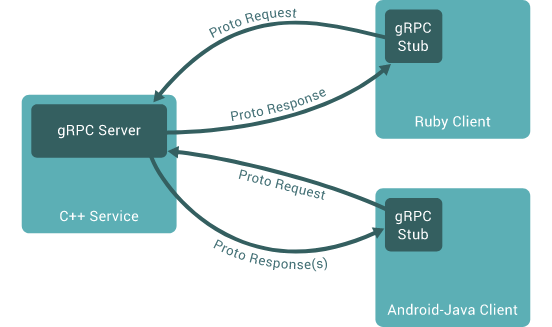
\includegraphics[width=\linewidth]{grpc.png}
    \caption{gRPC}
    \end{figure}
\paragraph{}
gRPC clients and servers can run and talk to each other in a variety of environments - from servers inside Google to your own desktop - and can be written in any of gRPC’s supported languages. So, for example, you can easily create a gRPC server in Java with clients in Go, Python, or Ruby. In addition, the latest Google APIs will have gRPC versions of their interfaces, letting you easily build Google functionality into your applications.

\begin{lstlisting}[caption= file.proto ]
syntax = "proto3";

package fileTransfer;

enum Status{
    ON_CREATE = 0;
    ON_UPLOAD = 1;
    ON_FINISH = 2;
}

message uploadByte{
    Status code = 1;
    string data = 2;
}

message status{
    Status code = 1;
}

service fileTransfer{
    rpc uploadFile (uploadByte) returns (status) {}
}
\end{lstlisting}

\section{Code}
\subsection{Client}
\begin{lstlisting}[language=javascript]
    const PROTO_PATH = __dirname + '/../protos/file.proto'
    const grpc = require('grpc')
    const fs = require('fs')
    const chunkingStreams = require('chunking-streams')
    const SizeChunker = chunkingStreams.SizeChunker
    const protoLoader = require('@grpc/proto-loader')
    const packageDefinition = protoLoader.loadSync(PROTO_PATH, { keepCase: true, longs: String, enums: String, defaults: true, oneofs: true })
    const fileTransfer_proto = grpc.loadPackageDefinition(packageDefinition).fileTransfer

    const client = new fileTransfer_proto.fileTransfer('localhost:8000', grpc.credentials.createInsecure())

    const filePath = __dirname + '/send/random.txt'
    const defaultSize = 10 * 1024
    const input = fs.createReadStream(filePath)
    const uploadFileProcess = async() => {
        client.uploadFile({ code: 0, data: "random.txt" }, (err, response) => {
            console.log(response.code)
            chunker = new SizeChunker({
                chunkSize: defaultSize,
                flushTail: true
            })
            chunker.on('data', (chunk) => {
                client.uploadFile({ code: 1, data: chunk.data.toString() }, (err, response) => {
                    console.log(response.code)
                })
            })
            input.pipe(chunker)
            input.on('end', () => {
                client.uploadFile({ code: 2, data: "" }, (err, response) => {
                    console.log(response.code)
                    input.close()
                })
            })
        })
    }
    uploadFileProcess()
\end{lstlisting}

\newpage

\subsection{Server}
\begin{lstlisting}[language=javascript]
    const PROTO_PATH = __dirname + '/../protos/file.proto'

    const grpc = require('grpc')
    const fs = require('fs')
    const protoLoader = require('@grpc/proto-loader')
    const packageDefinition = protoLoader.loadSync(PROTO_PATH, { keepCase: true, longs: String, enums: String, defaults: true, oneofs: true })
    const fileTransfer_proto = grpc.loadPackageDefinition(packageDefinition).fileTransfer
    
    var output;
    
    const uploadFile = (call, callback) => {
        switch (call.request.code) {
            case "ON_CREATE":
                output = fs.createWriteStream(`${call.request.data}`)
                callback(null, { code: call.request.code })
                break
            case "ON_UPLOAD":
                try {
                    output.write(Buffer.from(call.request.data))
                    callback(null, { code: call.request.code })
                } catch (err) {
                    console.log(err);
                }
                break
            case "ON_FINISH":
                callback(null, { code: call.request.code })
                break
        }
    }
    
    const server = new grpc.Server();
    server.addService(fileTransfer_proto.fileTransfer.service, { uploadFile: uploadFile })
    server.bind('localhost:8000', grpc.ServerCredentials.createInsecure())
    server.start()
\end{lstlisting}

\section{Who does what?}
    Bui Quang Huy : Research on gRPC and design nodejs app for RPC
    \newline
    Nguyen Viet Dung and Nguyen Quang Trung : Design and write the report.
    \newline
    Do Minh Hoang: Research about the protocol.
\end{document}


\end{document}